\section{Technical Design \& Analysis for Interface}

In this section. There will be analyzed some of the main features of the interface, and how they hold up in terms of time complexity.

\subsection{Interface}
A good way to improve performance when drawing the map, is to reduce the amount of things you draw every frame. When parsing the .OSM file, the different types of structures are split up into different types in the Type enum. Here they are assigned a hierarchy which is directly specified in the Type file. In earlier iterations of the program, some roads were assigned to a quite low hierarchy, which meant that they would only be drawn while the map was zoomed in a lot.\newline
In the end it was decided to move quite a lot of types a layer down in the hierarchy, as it vastly improved performance, since the program did not have to draw such a large amount of items. When zoomed further in, the KDTree allowed for better performance since most of the items outside the view simply were not drawn. 
There was much consideration when deciding which hierarchies the different types were assigned to. \\
The point when different hierarchies are drawn are hardcoded. They were changed throughout the different iterations of the program. 

\subsection{Zoombar}
One of the formal requirements stated that the program should include a graphical representation of the current zoom level. From that the following list of possible solutions came up:
\begin{itemize}
    \setlength{\itemsep}{0.2em}
    \item Displaying the current percentage of the zoom level
    \item Displaying the current range of a static ruler
\end{itemize}
The solution related to showing the current percentage of the zoom-level was ignored because of the disassociation with the value. Therefore, the first revision of our “zoom bar” was made by showing the width according to the map of a static picture of a ruler relative to the map. Which was made possible by using the haversine formula for calculating the distance.\\
After interacting with the program ourselves we decided to make the ruler that represents the distance to be dynamic, reasoned by the metric representation not being easily readable due to long obscure numbers and we liked the similar feature implemented in Google Maps. 
The dynamic zoom bar was set to have a class of its own, due to the benefits of securing low coupling and high cohesion.\\

\begin{wrapfigure}{r}{0.55\textwidth}
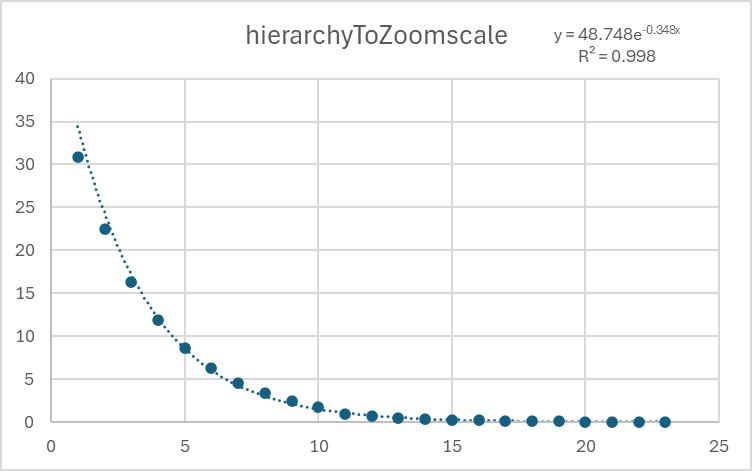
\includegraphics[width=1\linewidth]{docs/material/ZoomBar_Regression.png} 
\caption{Regression analysis of zoombar hierarchy levels}\label{zoombar/hierarchyLevelPicture}
\end{wrapfigure}

It is instantiated through its constructor requiring parameters such as: number of intervals, maximum zoom-level and minimum zoom-level. Due to the calculation of the dynamic zoom bar being compute intensive, we decided that the methods should be called during the loading of the map. These methods being \code{setZoombarScales()} and \code{setZoombarMetersInterval()}, which calculates the intervals at which zoom levels would indicate even numbers of meters. As illustrated in Figure \ref{zoombar/hierarchyLevelPicture}, both $X$ and $Y$ calculations are made by using exponential functions made from applying exponential regression to tables having zoom Level per mouse scroll. From that the amounts of mouse scrolls can be evenly distributed throughout the zoom intervals. Although this makes an imperfect representation of the distance, we deemed it to be accurate enough for our purposes. Next we have the hierarchy level to meters that determine how many meter options the zoom bar should have on runtime. Both allocated in the ram and secured that the calculation for the current amount of meters to be displayed on the zoom bar is cost efficient in runtime. It is calculated by calling setRange which does two things. It calls setZoombarHierarchyLevel that costs linear time to calculate what hierarchy level the current zoom amount corresponds to with a for loop $O(n)$, a comparison and an access of an array $O(1)$. Then setRange executes a return of an array access costing furthermore $O(1)$.
\begin{lstlisting}[language=Java, caption=Code of setZoombarHierarchyLevel()]
double hierarcyLevelToMeters(int lvl) 
    return 4.5925*Math.pow(Math.E, 0.7689*lvl);
\end{lstlisting}
\begin{table}[ht]
  \centering
  \begin{tabular}{ c|c }
& \textbf{Running time} \\ 
   \hline
   \textbf{Best case} & $\Omega (3)$ \\
   \textbf{Worst case} & $O(2+n)$ \\
  \end{tabular}\\
  \caption{\centering Zoombar's running time }\label{zoomBar/runnintime}
\end{table}